\documentclass[conference]{IEEEtran}
\IEEEoverridecommandlockouts
% The preceding line is only needed to identify funding in the first footnote. If that is unneeded, please comment it out.
\usepackage{cite}
\usepackage{amsmath,amssymb,amsfonts}
\usepackage{graphicx}
\usepackage{textcomp}
\usepackage{xcolor}
\usepackage{booktabs}
\usepackage{url}

\begin{document}

\title{Battery-Gated Measurement Validity in Wireless Sensor Deployments: Fault Characterisation, Recovery, and Downstream Consequences}

\author{
\IEEEauthorblockN{1\textsuperscript{st} Vasanth Iyer}
\IEEEauthorblockA{\textit{Dept. of Computer Science} \\
\textit{Grambling State University}\\
Grambling, LA, USA \\
iyerv@gram.edu}
\and
\IEEEauthorblockN{2\textsuperscript{nd} S. S. Iyengar}
\IEEEauthorblockA{\textit{Dept. of Computer \& Info. Science} \\
\textit{Florida International University}\\
Miami, FL, USA \\
iyengar@cis.fiu.edu}
\and
\IEEEauthorblockN{3\textsuperscript{rd} Vir Phoha}
\IEEEauthorblockA{\textit{Coll. of Eng. \& Computer Science} \\
\textit{Syracuse University}\\
Syracuse, NY, USA \\
email address or ORCID}
}

\maketitle

\begin{abstract}
Long-running wireless sensor deployments degrade as their batteries deplete,
and the resulting measurements can remain within physically plausible ranges
while being entirely uninformative. We characterise this failure on the Intel
Berkeley Research Lab deployment (54 motes, $2.3 \times 10^6$ readings) and
show that the conventional remedy---filtering readings by plausible
range---leaves the corruption intact in the evaluation window. Three results
follow. First, the fault is not a smooth voltage-dependent drift but a discrete
\emph{rail fault}: the converter saturates to a fixed $122.1^\circ$C with
humidity simultaneously railing negative, affecting $383{,}842$ readings.
Gating on battery voltage ($V \ge 2.4$~V) reduces the temperature standard
deviation from $12.42^\circ$C to $3.24^\circ$C, removing the corruption rather
than clipping it. Second, a voltage-free detector that fuses temperature,
humidity and light into a single Mahalanobis score independently validates the
gate---it identifies only four faults the gate misses in $2.2 \times 10^6$
readings---while showing the gate over-discards $8.59\%$ of readings; a
four-stage cleaner exploiting this recovers $10.9\%$ more data while
\emph{improving} accuracy by $3.6\%$. Third, the measurement-validity protocol
determines the outcome of downstream estimation: under range filtering, graph
message passing in a Kalman filter appears $13\%$ \emph{worse} than a
graph-free filter at reconstructing unobserved nodes, whereas under voltage
gating the same comparison reverses to a $27.1 \pm 2.9\%$ improvement. We
further characterise reconstruction of removed measurements, showing global
low-rank completion halves the error of graph harmonic extension, and quantify
the point at which undetected corruption defeats both. Applying the identical
estimator unchanged to human GPS mobility trajectories (taxi and private-car
trips, GeoLife dataset) reproduces the graph benefit and surfaces a second,
independent mechanism for protocol-dependent conclusions: taxi's fitted
coupling coefficient is the largest observed in either domain, yet is
invisible in a held-out test split that happens to contain no co-presence to
exercise it.
\end{abstract}

\begin{IEEEkeywords}
Measurement validity, sensor fault detection, wireless sensor networks, data
quality, Kalman filtering, matrix completion, battery depletion.
\end{IEEEkeywords}

\section{Introduction}

\IEEEPARstart{W}{ireless} sensor deployments intended to run unattended for
weeks or months are subject to a failure mode that conventional quality control
handles poorly. As a node's battery depletes, its measurements degrade
gradually and then catastrophically---but the degraded values need not leave
the physically plausible range, and so survive the range checks typically
applied before analysis. The consequence is not merely noisier data. Because
depletion correlates with time, and because evaluation splits in time-series
work are usually chronological, the corruption concentrates in precisely the
portion of the record reserved for evaluation.

Cleaning sensor streams is well studied---ensemble and stream-based models have
been proposed for precisely this setting~\cite{iyer2015}, and taxonomies of
sensor fault types are established~\cite{ni2009,sharma2010}. What has received
less attention is the \emph{consequence} of the cleaning choice: whether the
protocol adopted before analysis can alter, rather than merely degrade, the
conclusion drawn about a downstream method.

This paper characterises that failure on the Intel Berkeley Research Lab
deployment, the most widely used public wireless sensor dataset, and traces its
consequences through to a downstream estimation task. Our contributions are:

\begin{enumerate}
\item \textbf{Fault characterisation.} We show the corruption is a discrete
rail fault rather than a drift, identify its joint-channel signature, and
establish battery voltage as the causal index that separates valid from invalid
measurements (Section~\ref{sec:fault}).

\item \textbf{Independent validation.} We construct a detector that fuses the
three sensing channels without observing voltage, and use it together with a
spatial-consensus arbiter to establish that the voltage gate is sound as a
detector but over-conservative as an exclusion rule
(Section~\ref{sec:fusion}).

\item \textbf{A staged validity cleaner} that separates the two failure modes
present in the marginal voltage band, recovering $10.9\%$ more readings while
improving downstream accuracy (Section~\ref{sec:cleaner}).

\item \textbf{Demonstration that the protocol determines the conclusion.} On a
graph-based Kalman filtering task, the measured benefit of relational structure
reverses sign---from $13\%$ harmful to $27.1\%$ beneficial---according to which
validity protocol is applied (Section~\ref{sec:downstream}).

\item \textbf{Characterisation of recovery} for removed measurements, including
the regime boundaries between graph-local and global methods, their tolerance
to undetected corruption, and a locality-stratified account of accuracy and
precision (Sections~\ref{sec:recovery}--\ref{sec:locality}).

\item \textbf{External validity check.} We apply the identical graph
state-space model, unmodified, to human GPS mobility trajectories (taxi and
private-car trips, GeoLife dataset), showing the graph term again beats
persistence and finding a second, independent mechanism by which a real,
well-fitted effect can be invisible in a held-out test protocol
(Section~\ref{sec:external}).
\end{enumerate}

\section{Deployment and Measurement Chain}
\label{sec:deployment}

\subsection{Data}

The deployment comprises 54 Mica2Dot motes recording temperature, humidity,
light and battery voltage over 36 days from 28 February 2004, yielding
$2{,}313{,}682$ readings in the released file. Three mechanical issues require
attention before analysis. The \texttt{moteid} field contains out-of-range
values ($6485$, $33117$, $65407$) originating from corrupted packets;
$113{,}438$ duplicate \texttt{(moteid, epoch)} pairs are present; and the
\texttt{epoch} counter is 16-bit and wraps at $65535$, so it cannot serve as a
monotonic index across the record. We index by wall-clock timestamp. Sampling
is nominally $31$~s but irregular in practice (median $35.2$~s) and
unsynchronised across motes, so readings are resampled to a uniform five-minute
grid.

\subsection{Spatial structure}

\begin{figure}[t]
\centerline{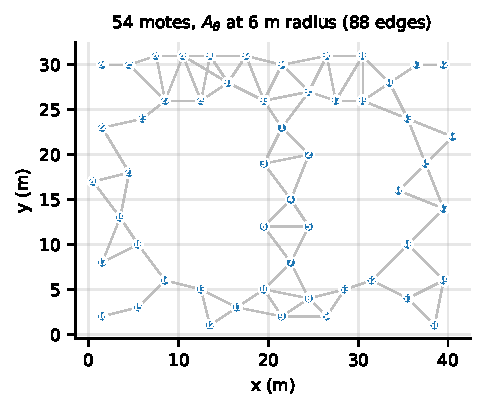
\includegraphics[width=\columnwidth]{figs/layout.pdf}}
\caption{The 54 motes at their published coordinates, with the adjacency
$A_\theta$ drawn at a 6~m connection radius. Six metres is the smallest radius
yielding a connected graph; at 5~m the network fragments into seven components
with two isolated motes.}
\label{fig:layout}
\end{figure}

The published mote coordinates permit an adjacency grounded in physical
geometry rather than inferred from the signal itself. Median nearest-neighbour
spacing is $3.6$~m over a $40.5 \times 31$~m floor. We threshold Euclidean
distance at $6$~m---the smallest radius leaving the graph connected---yielding
88 edges and mean degree $3.3$ (Fig.~\ref{fig:layout}).

\begin{figure}[t]
\centerline{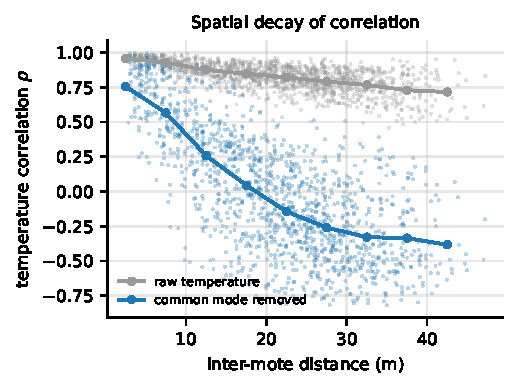
\includegraphics[width=\columnwidth]{figs/corrdist.pdf}}
\caption{Temperature correlation against inter-mote distance. Raw correlation
(grey) is nearly flat, being dominated by a building-wide diurnal cycle.
Removing the network-wide mean (blue) recovers the expected spatial decay.
Markers denote bin means.}
\label{fig:corrdist}
\end{figure}

Using geometry rather than signal correlation is deliberate.
Fig.~\ref{fig:corrdist} shows raw temperature correlation is nearly flat in
distance ($\rho = 0.739$ below $6$~m against $0.660$ beyond $30$~m;
distance--correlation $-0.10$), because a building-wide diurnal cycle dominates
every mote irrespective of separation. A correlation-thresholded graph overlaps
the spatial graph at Jaccard $0.08$. Removing the network-wide common mode
recovers the expected decay (distance--correlation $-0.48$). Since inferring
the graph from the signal one intends to predict is in any case circular, the
published coordinates are the sounder basis.

\subsection{Verification that spatial structure is recoverable}

\begin{figure}[t]
\centerline{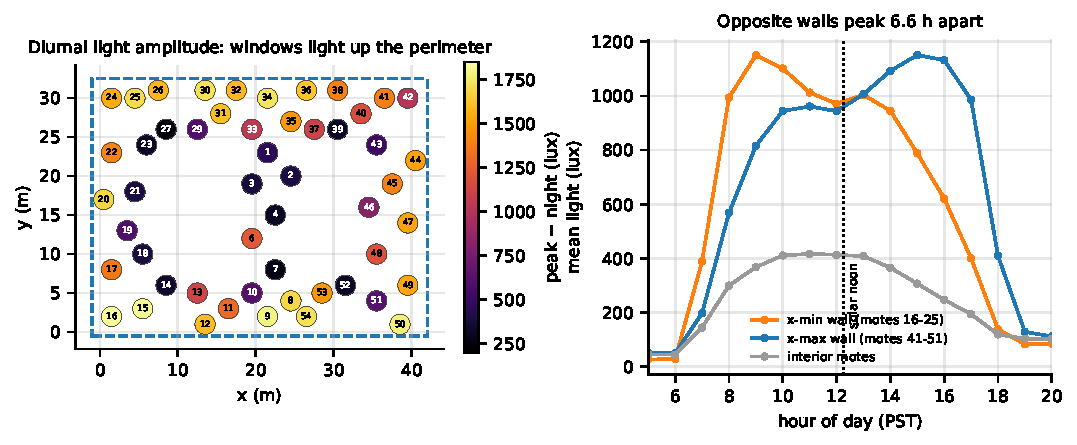
\includegraphics[width=\columnwidth]{figs/windows.pdf}}
\caption{Left: diurnal light amplitude by mote position; the perimeter is
clearly delineated. Right: mean light against hour of day for the two
$x$-extreme walls, which peak $6.6$~h apart.}
\label{fig:windows}
\end{figure}

As an independent check that the field carries the spatial structure the
adjacency assumes, we recover deployment geometry from the sensing channels
alone. Diurnal light amplitude (peak minus night baseline) correlates $-0.713$
with distance to the nearest wall: perimeter motes average $1569$~lux of swing
against $511$~lux for interior motes (Fig.~\ref{fig:windows}, left). Peak light
hour further separates the two $x$-extreme walls by $6.6$~h ($08{:}12$ against
$14{:}48$), the signature of opposite solar exposure, from which the building's
east--west axis can be identified---information absent from the published
coordinates, which are given in an arbitrary lab frame. Temperature confirms
this independently: diurnal swing correlates $-0.519$ with distance to wall
($7.24^\circ$C at the perimeter against $4.80^\circ$C inside). Two unrelated
channels agreeing supports treating spatial proximity as a meaningful prior.

\section{Fault Characterisation}
\label{sec:fault}

\subsection{Battery voltage indexes measurement validity}

\begin{table}[t]
\caption{Corruption as a function of battery voltage. ``Implausible'' denotes
temperature outside $[15,35]^\circ$C, an indoor office band.}
\label{tab:voltage}
\centering
\begin{tabular}{lrr}
\toprule
Voltage bin (V) & Readings & Implausible (\%) \\
\midrule
$(2.0, 2.2]$ & $232{,}194$ & $99.96$ \\
$(2.2, 2.3]$ & $169{,}129$ & $89.59$ \\
$(2.3, 2.4]$ & $221{,}805$ & $20.65$ \\
$(2.4, 2.5]$ & $398{,}154$ & $\mathbf{0.00}$ \\
$(2.5, 2.6]$ & $447{,}827$ & $0.22$ \\
$(2.6, 2.7]$ & $717{,}451$ & $0.29$ \\
\bottomrule
\end{tabular}
\end{table}

\begin{figure}[t]
\centerline{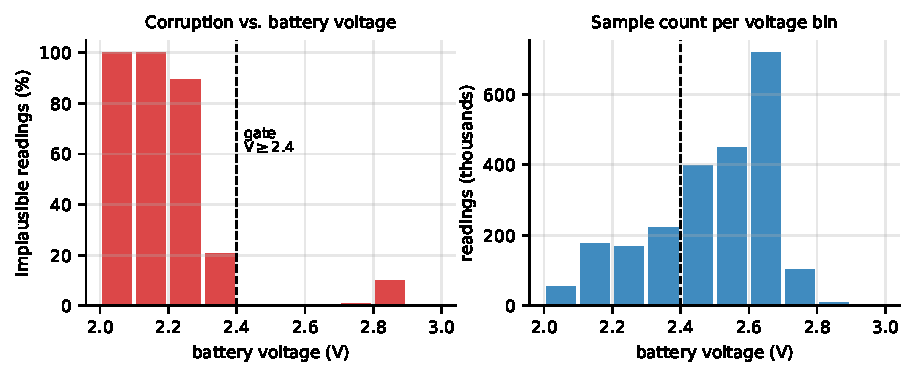
\includegraphics[width=\columnwidth]{figs/voltage.pdf}}
\caption{Left: fraction of implausible temperature readings against battery
voltage; the transition approximates a step at $2.4$~V. Right: sample counts
per bin.}
\label{fig:voltage}
\end{figure}

The temperature channel degrades as batteries deplete, reaching values as high
as $385^\circ$C. Table~\ref{tab:voltage} and Fig.~\ref{fig:voltage} show that
battery voltage separates valid from invalid readings far more sharply than the
readings separate themselves: below $2.3$~V almost every reading is
implausible, above $2.4$~V almost none is.

Gating at $V \ge 2.4$~V retains $72.8\%$ of readings and reduces the
implausible fraction to $0.30\%$. The decisive statistic is dispersion: the
temperature standard deviation falls from $12.42^\circ$C to $3.24^\circ$C. A
range filter cannot achieve this, because drifting readings that remain inside
$[0,50]^\circ$C survive it and silently contaminate the record.

\subsection{The fault is a rail, not a drift}

\begin{figure}[t]
\centerline{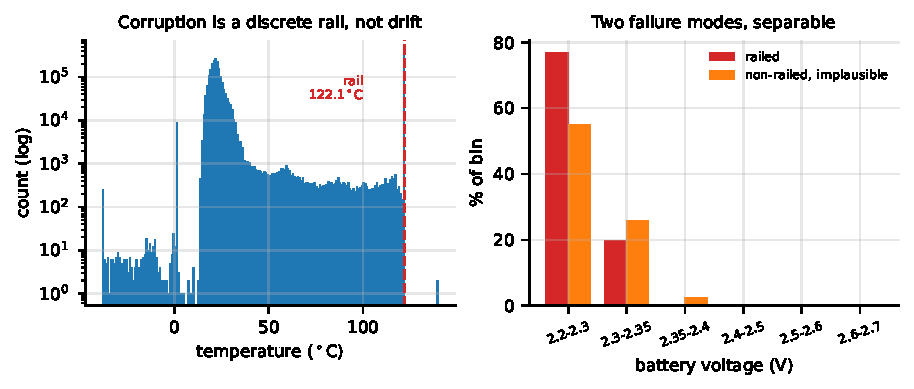
\includegraphics[width=\columnwidth]{figs/rail.pdf}}
\caption{Left: the temperature histogram is bimodal, exhibiting a discrete
spike at $122.1^\circ$C rather than a smeared drift---the converter saturates.
Right: split by rail status, the $(2.35, 2.40]$~V band is $0.12\%$ railed and
its survivors are $2.35\%$ implausible, as clean as the trusted region.}
\label{fig:rail}
\end{figure}

Fig.~\ref{fig:rail} establishes the mechanism. The corruption is not a smooth
voltage-dependent drift, which a calibration curve could invert, but a discrete
\emph{rail fault}: the converter saturates to a fixed $122.1^\circ$C while
humidity simultaneously rails negative. $383{,}842$ readings carry this joint
signature. A railed reading retains no recoverable information and cannot be
corrected---but it is deterministically detectable, which is what makes the
marginal band separable:

\begin{center}
\begin{tabular}{lrrr}
\toprule
Voltage (V) & $n$ & Railed & Non-railed implausible \\
\midrule
$(2.30, 2.35]$ & $105{,}941$ & $19.67\%$ & $25.97\%$ \\
$(2.35, 2.40]$ & $115{,}864$ & $0.12\%$ & $2.35\%$ \\
$(2.40, 2.50]$ & $398{,}154$ & $0.00\%$ & $0.00\%$ \\
\bottomrule
\end{tabular}
\end{center}

The $(2.35, 2.40]$ band is $0.12\%$ railed. It was being discarded for sharing
a bin edge with the genuinely broken data below it.

\subsection{Network attrition}

\begin{figure}[t]
\centerline{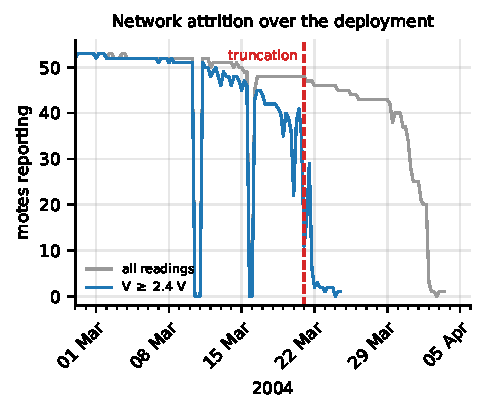
\includegraphics[width=\columnwidth]{figs/coverage.pdf}}
\caption{Motes reporting over time. The deployment decays progressively and is
effectively inactive after 23 March. A chronological $70/30$ split therefore
yields a test set that is only $5.4\%$ observed.}
\label{fig:coverage}
\end{figure}

A second hazard compounds the first. Motes drop out progressively
(Fig.~\ref{fig:coverage}) until essentially nothing reports. A chronological
$70/30$ split over the full record produces a test set with $5.4\%$ fill
against $80.9\%$ in training. We truncate to the window in which at least
$30\%$ of motes report, giving $6{,}521$ five-minute steps from 28 February to
21 March at $76.6\%$ fill.

\section{Independent Validation by Sensor Fusion}
\label{sec:fusion}

The voltage gate was derived from the data it screens and is therefore
self-justifying. This section constructs a second detector that never observes
voltage, and introduces a third arbiter---the spatial graph---to adjudicate
between them. Device-level trust may also be established cryptographically, for
instance through hardware-assisted authentication~\cite{bathalapalli2024}; the
approach taken here is complementary, inferring trustworthiness statistically
from the measurements themselves, and applies equally to archived data from
deployments that carry no such hardware. The adjudication step follows the
principle of resolving disagreement by census across independent
observers~\cite{iyer2022b}.

\subsection{A voltage-free fused validity score}

We fuse the three sensing channels into one scalar per reading via the
Mahalanobis distance in $(T, H, L)$, with location, robust scale and
correlation estimated on trusted readings:
\begin{equation}
s = \sqrt{z^\top C^{-1} z}, \qquad
z = (x - \mu) \oslash \sigma,
\label{eq:fused}
\end{equation}
with $\mu = [21.93^\circ\text{C}, 39.42\%, 165.6\ \text{lux}]$ and
$\sigma = [2.73, 6.03, 240.7]$ (scaled median absolute deviation). The physical
anchor is the temperature--humidity correlation of $-0.722$: indoor temperature
and relative humidity are strongly anti-correlated, so a reading violating that
relation is suspect even when each channel is individually within range. This
is what allows a single scalar to suffice.

\begin{figure}[t]
\centerline{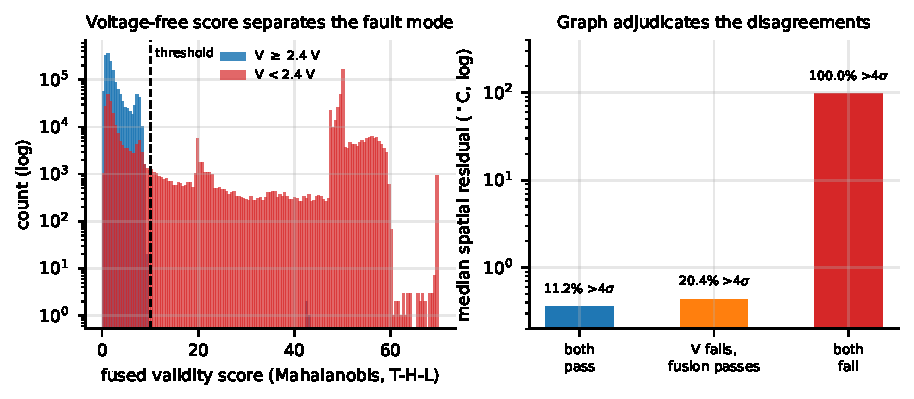
\includegraphics[width=\columnwidth]{figs/fusion.pdf}}
\caption{Left: the voltage-free fused score cleanly separates a healthy mode
from a fault mode, with the sub-threshold population concentrated in the
latter. Right: spatial residual for each agreement stratum; readings the
voltage rule rejects but fusion accepts resemble agreed-good data, not
agreed-bad data.}
\label{fig:fusion}
\end{figure}

Healthy readings ($V \ge 2.4$) have median score $1.59$; sub-threshold readings
$49.29$; railed readings $50.08$. The score attains AUC $0.9971$ against the
rail signature but only $0.8589$ against the voltage rule. That gap is
informative: the fused score reproduces the \emph{fault} almost perfectly while
only partly reproducing the \emph{rule}.

\subsection{Agreement and graph adjudication}

\begin{table}[t]
\caption{Agreement between the voltage rule and the voltage-free fused
detector, $n = 2{,}210{,}084$ readings.}
\label{tab:agree}
\centering
\begin{tabular}{lrr}
\toprule
 & Fusion pass & Fusion fail \\
\midrule
$V \ge 2.4$ (pass) & $1{,}608{,}565$ & $4$ \\
$V < 2.4$ (fail)   & $189{,}843$ & $411{,}672$ \\
\bottomrule
\end{tabular}
\end{table}

\begin{table}[t]
\caption{Spatial residual against healthy neighbours for each agreement
stratum (null standard deviation $0.326^\circ$C).}
\label{tab:adjudicate}
\centering
\begin{tabular}{lrrr}
\toprule
Stratum & $n$ & Median $|r|$ & Beyond $4\sigma$ \\
\midrule
Both pass                  & $236{,}405$ & $0.358^\circ$C & $11.2\%$ \\
$V$ fails, fusion passes   & $5{,}746$ & $0.436^\circ$C & $20.4\%$ \\
Both fail                  & $2{,}011$ & $97.268^\circ$C & $100.0\%$ \\
\bottomrule
\end{tabular}
\end{table}

Table~\ref{tab:agree} shows the two detectors agree on $91.41\%$ of readings.
Critically, the voltage gate misses almost nothing: only four readings in
$2.2 \times 10^6$ pass the voltage rule while failing fusion. But it rejects
$189{,}843$ readings ($8.59\%$) that the sensing channels consider valid.

Table~\ref{tab:adjudicate} adjudicates these disagreements using the spatial
graph, which is independent of both detectors. The over-discarded readings have
median residual $0.436^\circ$C, close to agreed-good data ($0.358^\circ$C) and
far from agreed-bad data ($97.268^\circ$C). They are usable, if modestly
noisier ($20.4\%$ against $11.2\%$ beyond $4\sigma$).

The conclusion is twofold and is what motivates Section~\ref{sec:cleaner}: the
voltage gate is \emph{validated as a detector} and \emph{refuted as an
exclusion rule}, by an instrument sharing no information with the rule it
evaluates.

\subsection{Two negative results}

Two natural hypotheses do not survive testing, and we report them because each
would otherwise be an attractive design choice.

\textbf{Fault simultaneity is not a common-cause event, but only phase
conditioning reveals this.} Pooled over the record, $35.7\%$ of $30$-minute
windows exhibit more than eight simultaneous faults, suggesting system-level
failure. Conditioned on deployment phase, the picture inverts: before 15 March,
$63\%$ of windows are fault-free and $95.5\%$ of those containing a fault
involve exactly one mote, with none exceeding eight; after 15 March, only $2\%$
are fault-free and $67.1\%$ involve more than eight, with median faulty
fraction $0.93$. Early faults are isolated device failures; late co-occurrence
is correlated end-of-life as batteries deplete together. The pooled statistic
would mislead.

\textbf{Fusion provides no early warning.} Voltage crosses $2.4$~V before the
sensing channels corrupt in 47 of 51 motes, with median lead $3.0$ days. The
sensing channels are downstream of the battery, so the fused score confirms the
causal mechanism rather than anticipating it. Where early warning is the
objective, voltage is already the best available signal.

\section{A Staged Validity Cleaner}
\label{sec:cleaner}

Section~\ref{sec:fusion} established that the voltage cutoff over-discards.
We therefore replace it with a four-stage procedure. The staging follows the
ensemble principle applied to sensor-stream cleaning in~\cite{iyer2015}, in
which independent weak tests are composed rather than a single decision
boundary being tuned; here the tests are deliberately heterogeneous---one
deterministic, one distributional, one relational, one probabilistic---so that
their failure modes do not coincide.

\begin{enumerate}
\item[S1] \textbf{Rail detection.} Deterministic joint-channel test:
$|T - 122.13| < 0.05$ or $H < 0$. No threshold tuning is required.
\item[S2] \textbf{Validity bounds.} A physical-range guard, tightened using the
agreed-healthy population (Section~\ref{sec:bounds}).
\item[S3] \textbf{Graph consensus.} Each surviving candidate is compared
against the median of its \emph{trusted} neighbours at the same timestamp. The
null is calibrated on trusted data only, so the threshold does not inherit
contamination from the candidates it screens; the resulting robust spatial
residual standard deviation is $0.518^\circ$C, and candidates beyond
$\tau\sigma$ are rejected.
\item[S4] \textbf{Heteroscedastic measurement noise.} Surviving marginal
readings enter downstream estimation with an inflated noise variance rather
than being accepted or rejected outright.
\end{enumerate}

That recovered readings are genuinely sound, rather than merely plausible, is
confirmed by their spatial residual: $0.503^\circ$C for the $(2.35, 2.40]$~V
band against $0.467$--$0.493^\circ$C for trusted readings.

\subsection{Tightened validity bounds}
\label{sec:bounds}

\begin{table}[t]
\caption{Detections beyond the a-priori box, adjudicated by the graph (null
standard deviation $0.326^\circ$C).}
\label{tab:bounds}
\centering
\begin{tabular}{lrrr}
\toprule
Rule & Caught & Median $|r|$ & Beyond $4\sigma$ \\
\midrule
Empirical box ($T,H$)      & $697$ & $3.285^\circ$C & $79.2\%$ \\
$T$--$H$ ellipse           & $532$ & $8.954^\circ$C & $87.2\%$ \\
Box $\cup$ ellipse         & $\mathbf{900}$ & $6.323^\circ$C & $\mathbf{81.6\%}$ \\
\midrule
Retained (combined)        & $241{,}210$ & $0.359^\circ$C & $11.2\%$ \\
Retained (a-priori box)    & $242{,}110$ & $0.361^\circ$C & $11.4\%$ \\
\bottomrule
\end{tabular}
\end{table}

The a-priori guard $T \in [10,45]^\circ$C, $H \in [0,100]\%$ is loose. We
calibrate tighter bounds on readings both detectors accept, at $99.9\%$
coverage, which bounds false rejection on good data at $0.1\%$ by construction.

We note that the correlation-aware region is \emph{not} tighter by volume than
a percentile box: at matched coverage the empirical box occupies $0.205$ of the
a-priori volume against $0.923$ for the fused ellipsoid, because the light
channel is wide-ranging and weakly correlated with the others. Restricting to
the $(T,H)$ subspace does not reverse this (box $847.2$ against ellipse
$890.6$). Volume, however, is the wrong figure of merit.
Table~\ref{tab:bounds} shows both rules detect genuine faults---$79$--$87\%$ of
flagged readings lie beyond $4\sigma$ against a baseline of $11.4\%$---and that
they catch overlapping but non-identical sets. The ellipse contributes
approximately $200$ detections no axis-aligned bound can find: the physically
impossible hot-and-humid and cold-and-dry combinations. The cost is $0.37\%$ of
retained data with residual essentially unchanged. The recommended S2 rule is
therefore the disjunction
\begin{equation}
T \notin [14.58, 35.91]\ \lor\ H \notin [16.08, 55.79]\ \lor\ m_{TH} > 4.99 .
\end{equation}

\subsection{Result}

\begin{table}[t]
\caption{Staged cleaner against the hard voltage cutoff.}
\label{tab:staged}
\centering
\begin{tabular}{lrrr}
\toprule
 & Cutoff & Staged & Change \\
\midrule
Rows retained     & $1{,}677{,}047$ & $1{,}860{,}173$ & $+10.9\%$ \\
Grid cells        & $269{,}943$ & $294{,}803$ & $+9.2\%$ \\
Usable window     & $5{,}996$ & $6{,}390$ steps & $+33$~h \\
Imputation RMSE   & $2.147^\circ$C & $\mathbf{2.070^\circ}$\textbf{C} & $-3.6\%$ \\
\bottomrule
\end{tabular}
\end{table}

Table~\ref{tab:staged} shows the cleaner is denser \emph{and} more accurate:
whatever additional noise the recovered readings carry, the density gain more
than repays it. We note that S4 is inert at the operating point used here
($R_0 = 10^{-4}$ in standardised units, where process noise dominates); it is
retained because it becomes load-bearing at larger $R$.

\section{Downstream Consequence}
\label{sec:downstream}

We now show that the validity protocol, not the estimator, determines the
conclusion one draws about a downstream method.

\subsection{Estimator}

We adopt the graph state-space formulation of~\cite{alippi2023}, in which
inputs, states and outputs are attributed graphs. For a fixed deployment the
time-varying-topology machinery is inactive and the model reduces to
\begin{equation}
s_t = \theta_{tm} s_{t-1} + \theta_{sp} \bar{A}_\theta s_{t-1} + \eta_{t-1},
\qquad y_t = s_t + \nu_t,
\label{eq:model}
\end{equation}
with $\bar{A}_\theta = D^{-1/2}(I + A_\theta) D^{-1/2}$, identity readout, and
$\theta$ fitted by least squares on the training split. The transition being
linear, the filter is an exact Kalman filter. Setting $\theta_{sp} = 0$ yields
the graph-free ablation. The error covariance
$P_t \in \mathbb{R}^{|V| \times |V|}$ is a covariance \emph{across nodes}: its
off-diagonal entries are the only channel by which an observation at one mote
informs the estimate at another.

\subsection{The conclusion reverses}

\begin{table}[t]
\caption{One-step-ahead ($5$~min) prediction RMSE at observed nodes.}
\label{tab:onestep}
\centering
\begin{tabular}{lc}
\toprule
Model & RMSE ($^\circ$C) \\
\midrule
Persistence & $0.269$ \\
KF, no graph ($\theta_{sp} = 0$) & $0.275$ \\
KF, graph message passing & $\mathbf{0.262}$ \\
\bottomrule
\end{tabular}
\end{table}

\begin{table}[t]
\caption{Imputation RMSE for never-observed motes ($9$ of $39$ withheld), mean
over $10$ random draws. The protocols differ only in the validity rule.}
\label{tab:holdout}
\centering
\begin{tabular}{lccc}
\toprule
Validity protocol & No graph & Graph MP & Change \\
\midrule
Range filter $[0,50]^\circ$C & $3.875$ & $4.377$ & $+13.0\%$ \\
Voltage gate $V \ge 2.4$~V & $2.519$ & $\mathbf{1.833}$ & $\mathbf{-27.1\%}$ \\
\bottomrule
\end{tabular}
\end{table}

\begin{figure}[t]
\centerline{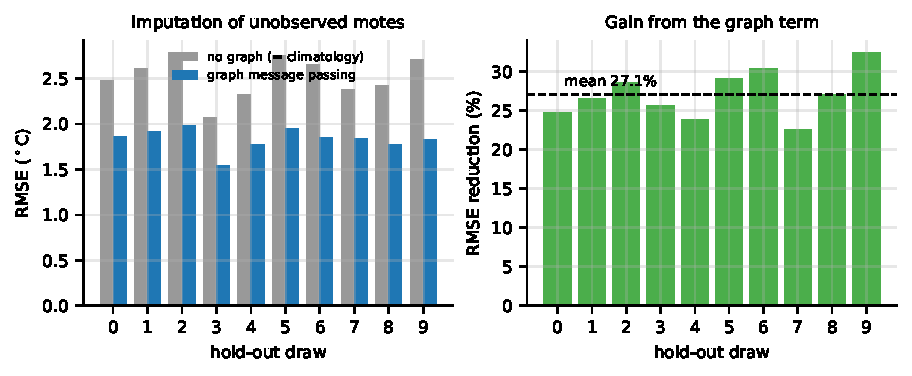
\includegraphics[width=\columnwidth]{figs/holdout.pdf}}
\caption{Left: imputation RMSE per hold-out draw. Right: RMSE reduction
attributable to the graph term, mean $27.1\%$, positive in all ten draws.}
\label{fig:holdout}
\end{figure}

\begin{figure*}[t]
\centerline{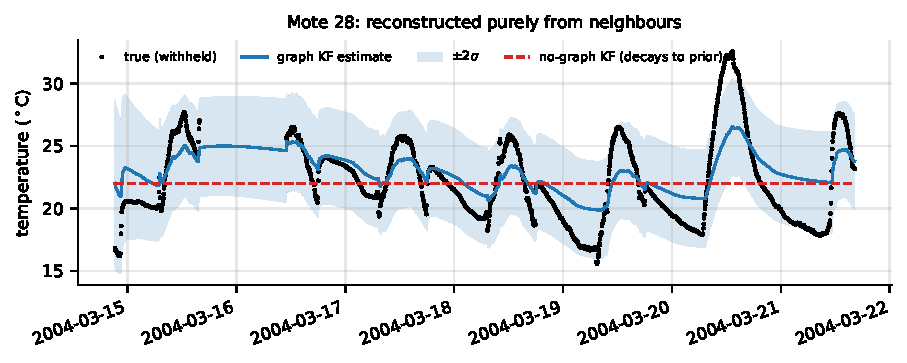
\includegraphics[width=0.86\textwidth]{figs/trace.pdf}}
\caption{Mote 28, withheld from the filter for the entire test period and
reconstructed from its neighbours through the state-transition graph. The
graph-free filter (red, dashed) decays to the prior mean because no measurement
can reach the node; the graph filter (blue) tracks the withheld signal, with
the shaded band showing $\pm 2\sigma$ from the propagated covariance.}
\label{fig:trace}
\end{figure*}

Table~\ref{tab:holdout} is the central result. Under the range filter, the
graph term \emph{degrades} performance by $13\%$; under the voltage gate, the
identical comparison shows a $27.1 \pm 2.9\%$ improvement, favouring the graph
in all ten draws (Fig.~\ref{fig:holdout}). The conclusion one would draw about
the method reverses on a measurement-validity choice.

The graph-free filter matches climatology to three decimal places, and
necessarily so: with no measurement ever reaching a withheld node, its estimate
decays to the prior mean. Fig.~\ref{fig:trace} shows this directly.

Table~\ref{tab:onestep} shows the benefit is confined to unobserved nodes; at
observed nodes the graph term is worth under $5\%$. The fitted parameters
explain why: $\theta_{tm} = 0.992$ against $\theta_{sp} = 0.0064$. At a
five-minute cadence indoor temperature is a near-perfect random walk, so a
mote's own previous reading is very nearly a sufficient statistic.

\section{Recovery of Removed Measurements}
\label{sec:recovery}

Railed readings are removed, not corrected. We characterise their
reconstruction.

\subsection{Graph harmonic extension}

Zeroing removed cells and iterating neighbour averaging with observed nodes
clamped converges to the harmonic extension---the minimiser of the Dirichlet
energy $\sum_{uv} w_{uv}(x_u - x_v)^2$ subject to the observed boundary. Three
properties hold empirically. Initialisation is irrelevant: zeros, climatology,
random $\mathcal{N}(0,3)$ and a $+100$ offset converge to the same fixed point
to within $2.8 \times 10^{-17}$. The clamp is essential: leaving zeroed cells
in as sources degrades RMSE from $0.484$ to $1.923^\circ$C and collapses the
field to standard deviation $0.024^\circ$C. Convergence is fast, the maximum
per-iteration update falling below $10^{-3}$ by iteration $8$.

Capacity degrades gracefully: at $80\%$ of nodes blank, harmonic extension
achieves $1.14^\circ$C against $3.32^\circ$C for climatology and
$2.40^\circ$C for single-hop averaging (Fig.~\ref{fig:capacity}, left).

\subsection{Global low-rank completion}

\begin{figure}[t]
\centerline{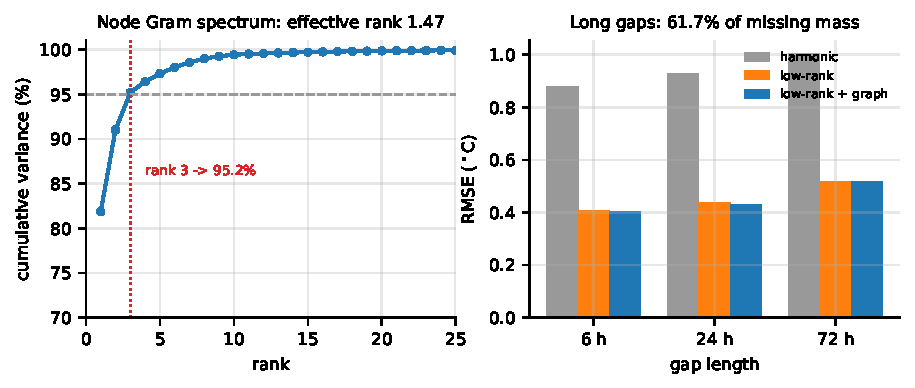
\includegraphics[width=\columnwidth]{figs/lowrank.pdf}}
\caption{Left: the node Gram spectrum is dominated by one mode; rank 3 captures
$95.2\%$ of variance and the effective rank is $1.47$ of $41$. Right: on long
gaps, which carry $61.7\%$ of all missing cells, low-rank completion
approximately halves the error of harmonic extension.}
\label{fig:lowrank}
\end{figure}

\begin{table}[t]
\caption{Reconstruction RMSE under missingness sampled from the empirical
gap-length distribution ($30\%$, mean of 3 draws).}
\label{tab:lowrank}
\centering
\begin{tabular}{lc}
\toprule
Method & RMSE ($^\circ$C) \\
\midrule
Climatology & $3.137$ \\
Harmonic extension & $0.926$ \\
Low-rank ALS & $0.475$ \\
Low-rank $+$ graph prior & $\mathbf{0.452}$ \\
\bottomrule
\end{tabular}
\end{table}

The field is very low rank: rank~1 explains $81.9\%$ of variance, rank~3
$95.2\%$, with effective rank $1.47$ of $41$ (Fig.~\ref{fig:lowrank}, left).
Factorising $X \approx UV^\top$ and minimising
\begin{equation}
\|K \circ (UV^\top + b - Y)\|^2 + \alpha(\|U\|^2 + \|V\|^2)
+ \lambda_g \operatorname{tr}(V^\top L V)
\label{eq:lowrank}
\end{equation}
gives a $51.2\%$ reduction over harmonic extension
(Table~\ref{tab:lowrank}). We note this must be optimised by alternating least
squares rather than a generic first-order method; Adam produced non-monotone
behaviour in the rank ($r{=}3$: $0.898$, $r{=}8$: $1.407$, $r{=}12$: $0.550$),
which is optimiser noise rather than a property of the model.

The method has one clean failure mode. For nodes observed at \emph{no}
timestamp, plain low-rank collapses to climatology ($3.438$ against $3.454$),
as such a node has no data constraining its loading $V_j$. The graph prior
supplies one and recovers much of the loss ($1.307$), but harmonic extension
still wins outright ($0.825$). The two are complementary, and we route by
observability. Reconstruction from an under-determined observation set is
ill-posed in the same sense encountered in edge re-identification
tasks~\cite{iyer2022}, and is likewise resolved by imposing structure---here a
low-rank factorisation and a graph prior---rather than by additional data.

\section{Limits: Tolerance to Undetected Corruption}
\label{sec:byzantine}

\begin{figure}[t]
\centerline{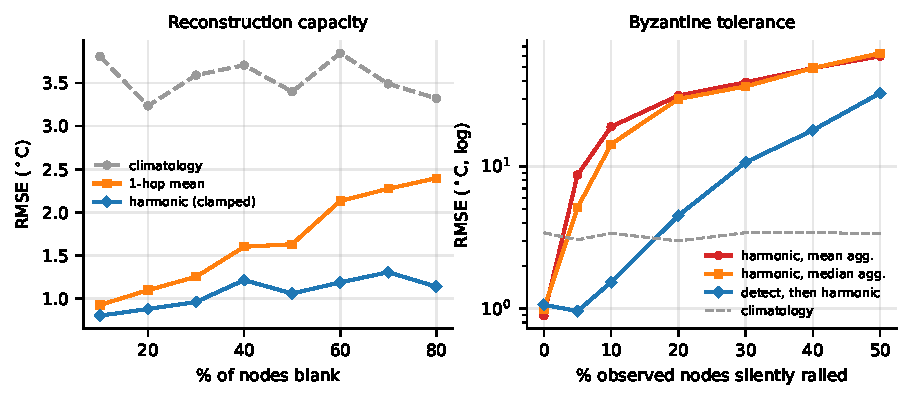
\includegraphics[width=\columnwidth]{figs/capacity_byz.pdf}}
\caption{Left: reconstruction RMSE against the fraction of blank nodes. Right:
RMSE at reconstructed nodes as observed nodes are silently railed (log scale).
Robust aggregation does not avert the collapse; detection does.}
\label{fig:capacity}
\end{figure}

\begin{table}[t]
\caption{RMSE ($^\circ$C) at reconstructed nodes with $30\%$ of nodes blank, as
a fraction of the \emph{observed} nodes is silently railed and treated as
trustworthy.}
\label{tab:byzantine}
\centering
\begin{tabular}{lrrrr}
\toprule
Corrupt & Mean agg. & Median agg. & Detect first & Climatology \\
\midrule
$0\%$  & $0.892$ & $0.992$ & $1.064$ & $3.418$ \\
$5\%$  & $8.724$ & $5.123$ & $\mathbf{0.960}$ & $3.049$ \\
$10\%$ & $19.067$ & $14.367$ & $\mathbf{1.535}$ & $3.390$ \\
$20\%$ & $31.587$ & $29.871$ & $4.516$ & $2.993$ \\
$50\%$ & $59.732$ & $62.791$ & $32.884$ & $3.363$ \\
\bottomrule
\end{tabular}
\end{table}

Table~\ref{tab:byzantine} quantifies what happens when detection fails. A
railed node lies some $30$ standard deviations from the field, and the harmonic
solution is a weighted average of \emph{all} boundary values, so local damage
becomes global. At $5\%$ undetected corruption, reconstruction is already
$2.9\times$ worse than predicting the global mean.

Robust aggregation is not an adequate remedy: median aggregation recovers only
a factor of approximately $1.4$ and is itself worse than climatology from $5\%$
onward. The reason is that the breakdown point is \emph{local}. A median
tolerates corruption below half of each node's own neighbourhood, and this
graph is sparse---mean degree $3.3$, with 13 of 54 motes unable to outvote even
one corrupted neighbour. A $5\%$ global fraction therefore concentrates into a
local majority somewhere in the graph with near certainty, and the classical
$n \ge 3f+1$ intuition misleads: the relevant quorum is the neighbourhood, not
the network.

This is an empirical counterpart to the aggregation lower bounds derived
in~\cite{iyer2026}, where the attainable precision of distributed sensor fusion
under Byzantine faults is shown to be governed by the structure over which
aggregation occurs rather than by the global fault fraction alone. The present
measurements make the same point concretely for a physical deployment: the
governing quantity is the degree distribution, and reporting a network-wide
tolerance figure without it would overstate robustness by an order of
magnitude.

Screening before reconstruction holds RMSE at $0.96$--$1.54^\circ$C through
$10\%$ contamination, an order of magnitude better than robust aggregation.
This is the operational justification for the deterministic S1 test.

\section{Locality-Stratified Accuracy and Precision}
\label{sec:locality}

\begin{figure}[t]
\centerline{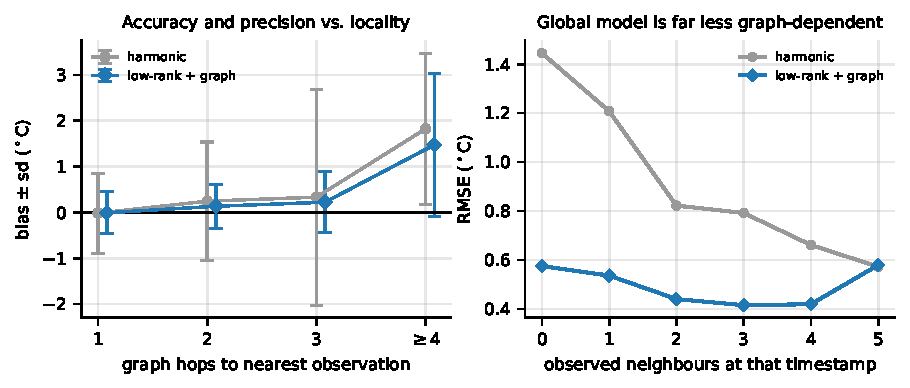
\includegraphics[width=\columnwidth]{figs/locality.pdf}}
\caption{Left: bias $\pm$ standard deviation against graph-hop distance to the
nearest observation. Right: RMSE against the number of observed neighbours.}
\label{fig:locality}
\end{figure}

\begin{table}[t]
\caption{Bias / standard deviation / RMSE ($^\circ$C) by graph-hop distance to
the nearest observed node.}
\label{tab:locality}
\centering
\begin{tabular}{lrcc}
\toprule
Hops & $n$ & Harmonic & Low-rank $+$ graph \\
\midrule
$1$      & $58{,}387$ & $-0.015$ / $0.873$ / $0.873$ & $-0.007$ / $0.458$ / $\mathbf{0.458}$ \\
$2$      & $4{,}384$  & $+0.246$ / $1.291$ / $1.315$ & $+0.135$ / $0.484$ / $\mathbf{0.502}$ \\
$3$      & $370$      & $+0.334$ / $2.358$ / $2.382$ & $+0.224$ / $0.670$ / $\mathbf{0.706}$ \\
$\geq 4$ & $65$       & $+1.826$ / $1.650$ / $2.461$ & $+1.476$ / $1.561$ / $2.149$ \\
\bottomrule
\end{tabular}
\end{table}

Aggregate RMSE obscures how error relates to local graph context. Reporting
accuracy (bias) and precision (standard deviation) separately
(Table~\ref{tab:locality}, Fig.~\ref{fig:locality}) yields three observations.

The graph is a strong hypothesis for the local method and a weak one for the
global method: harmonic error grows $2.7\times$ from one hop to three, low-rank
only $1.5\times$. A global model reaches an isolated node through the shared
factor rather than through the graph.

Accuracy and precision degrade differently, and only bias is
graph-directional. Bias is near zero at two to four observed neighbours and
turns positive as the neighbourhood empties, isolated reconstructions being
pulled toward the field mean. Precision degrades monotonically with isolation
for harmonic ($0.516 \to 1.419$) but is nearly flat for low-rank
($0.414 \to 0.552$).

Graph position nonetheless predicts an individual cell's error poorly:
correlation between absolute error and hop distance is $+0.089$ for harmonic
and $+0.138$ for low-rank. Graph context shifts the error \emph{distribution}
substantially while predicting any single cell weakly, so a per-cell confidence
interval derived from graph position alone would be poorly calibrated. The
$\geq\!4$-hop stratum contains only $65$ cells and should be read as
indicative.

\section{External Validity: Human Mobility Trajectories}
\label{sec:external}

Section~\ref{sec:downstream} showed that the graph term's apparent benefit
depends on the measurement-validity protocol applied before evaluation, on a
single wireless deployment. This raises a natural follow-up question: is the
effect specific to that deployment, or does the same linear graph state-space
model (Eq.~\ref{eq:model}) generalise to a structurally different sensing
domain? We apply it unchanged to human GPS mobility trajectories, substituting
position $(x,y)$ for $(T,H,L)$ and co-presence for spatial adjacency.

\subsection{Setup}

We use GeoLife~\cite{zheng2010geolife}, GPS logs from users in and around
Beijing, restricted to the 28 users carrying transportation-mode labels, a
50-day busiest-activity subset, and the Beijing metropolitan bounding box.
Raw points are resampled onto a common absolute 5-second grid so different
users' trajectories are directly time-comparable, then cut into
non-overlapping 100-second windows (8 observed steps, 12 held out), following
the observation/prediction convention of
TrajImpute~\cite{chib2024trajimpute}. Two windows sharing a global time index
are a candidate scene; an edge is added when the pair's mean position over the
window is within 50~m, the radius separating genuine co-presence from
same-clock-time coincidence in this data. $\theta$ is fit per transportation
mode by the same pooled least-squares procedure used for the deployment
(Section~\ref{sec:downstream}), on a 70/15/15 user-disjoint split. Missingness
is simulated on the 8 observed steps under the same Easy
($m \sim \mathcal{U}\{0,\ldots,4\}$) / Hard ($m \sim \mathcal{U}\{4,\ldots,7\}$)
protocols as TrajImpute. Unlike the deployment, there is no faulty
subpopulation to gate against here, so this check isolates the estimator's
behaviour from the fault-detection question addressed in
Sections~\ref{sec:fault}--\ref{sec:cleaner}.

We report the two modes most relevant to a fleet-of-vehicles reading of the
deployment result: private car and taxi. The two were initially merged, as
the GeoLife label guide groups both under a single ``driving'' category;
splitting them changes the private-car numbers materially, evidence the two
populations follow different dynamics. Walk, bus, bike and subway were also
tested and show the same qualitative pattern (graph beating persistence) but
are not reported in detail here.

\subsection{Results}

\begin{table}[t]
\caption{Graph-message-passing generalisation to GeoLife taxi and
private-car trajectories (position MAE, metres).}
\label{tab:geolife}
\centering
\begin{tabular}{llrrrr}
\toprule
Mode & Protocol & No graph & Graph MP & Persist. & $\theta_{sp}$ \\
\midrule
Car (private) & Easy & $26.714$ & $\mathbf{26.709}$ & $27.249$ & $+0.0130$ \\
Car (private) & Hard & $47.274$ & $\mathbf{47.257}$ & $47.896$ & $+0.0130$ \\
Taxi          & Easy & $35.629$ & $\mathbf{35.617}$ & $36.486$ & $+0.0626$ \\
Taxi          & Hard & $59.555$ & $\mathbf{59.546}$ & $60.274$ & $+0.0626$ \\
\bottomrule
\end{tabular}
\end{table}

Table~\ref{tab:geolife} shows the graph term beats persistence in both modes
and both protocols, consistent with the deployment's positive result under
its own (voltage-gated) validity protocol. Taxi's fitted
$\theta_{sp} = 0.0626$ is the largest graph-coupling coefficient obtained
anywhere in this study---roughly $5\times$ the deployment's $0.0064$
(Section~\ref{sec:downstream}) and $4.8\times$ private car's $0.0130$---
consistent with commercially dispatched vehicles sharing traffic-flow
correlations more tightly than private trips or a fixed indoor deployment.

This coefficient is fit from ten genuine co-presence scenes among seven
training users. But the user-disjoint test split places only two
taxi-labelled users in the held-out set, and they never co-occur: all $261$
test scenes are singletons, so the fitted graph term has no edge to act on
during evaluation. The resulting test-set MAE improvement ($0.03\%$) is
negligible despite the underlying coefficient being an order of magnitude
larger than any other mode's.

\subsection{A second illustration of protocol-dependence}

This is a second, independent demonstration of the paper's central claim,
arrived at by a different mechanism. Section~\ref{sec:downstream} showed the
measurement-validity rule determines whether a real graph benefit is visible.
Here, the composition of the evaluation split plays the analogous role: a
coefficient fit correctly and substantially from training data can be
invisible in a held-out test metric purely because that split happens to
contain no instance of the structure the coefficient encodes. A negative or
near-null result at test time does not certify the absence of the effect
being measured in either case---only that the evaluation protocol failed to
exercise it.

\section{Discussion}

\textbf{Measurement-validity protocol can dominate methodological effect.} The
difference between the two rows of Table~\ref{tab:holdout} exceeds any
difference we observed between estimator variants. Where a corruption mechanism
is physically indexed, gating on that index is not housekeeping---it decides
the result. The same hazard should be expected wherever sensor degradation
correlates with time and evaluation splits are chronological.

\textbf{Detectors should be validated against instruments that do not share
their information.} The voltage gate appeared sound in isolation; only a
voltage-free detector could establish that it misses almost nothing, and only a
third arbiter could establish that its rejections were largely unwarranted.
Reporting a validity rule without such a check leaves its false-rejection rate
unmeasured.

\textbf{Detection and reconstruction are not interchangeable.} It is tempting
to treat sufficiently robust reconstruction as a substitute for identifying bad
data. Table~\ref{tab:byzantine} shows otherwise on a sparse graph: corruption a
deterministic detector removes exactly will defeat a median aggregator at $5\%$
prevalence, because the aggregator's quorum is a neighbourhood of three rather
than a network of $54$.

\textbf{Limitations.} We fit the two-parameter linear model
of~\eqref{eq:model} rather than a nonlinear spatio-temporal graph network, so
the $27.1\%$ should be read as a lower bound on what the architecture can
deliver. The $6$~m radius was fixed a priori from connectivity and not tuned
against the hold-out objective. The tightened bounds of
Section~\ref{sec:bounds} encode this building's operating envelope over five
late-winter weeks, not a sensor specification; the method transfers, the
constants do not. Finally, the dataset's published radio-connectivity file
offers an adjacency grounded in measured link quality rather than Euclidean
distance, which would be a natural comparison. The GeoLife check
(Section~\ref{sec:external}) is similarly bounded: 28 labelled users, 50
days, Beijing only, and as few as two users in some held-out splits; we
report taxi and private car as the modes most relevant to a fleet-vehicle
reading of the deployment result.

\section{Conclusion}

We characterised battery-gated measurement validity on a widely used wireless
sensor deployment and traced its consequences downstream. The corruption is a
discrete rail fault rather than a drift, indexed causally by battery voltage,
and a voltage-free fusion detector independently confirms the gate misses
almost nothing while over-discarding $8.59\%$ of readings. A staged cleaner
exploiting this recovers $10.9\%$ more data and improves accuracy $3.6\%$.

Most consequentially, the choice of validity protocol reverses the sign of a
downstream methodological conclusion: relational structure in a graph Kalman
filter appears $13\%$ harmful under range filtering and $27.1 \pm 2.9\%$
beneficial under voltage gating. For practitioners, the measurement-validity
rule belongs in the ablation table alongside the model.

The same conclusion holds beyond this deployment. Applying the identical
model to human GPS trajectories (taxi and private-car mobility) reproduces
the graph benefit, and a well-fitted coupling coefficient---the largest
observed in either domain---can still be invisible in a held-out split that
contains no instance of the structure it encodes: a second, independent
route to the same protocol-dependence identified in this paper.

\section*{Data Availability}

The Intel Berkeley Research Lab dataset, comprising both readings and mote
coordinates, is publicly available at
\url{https://db.csail.mit.edu/labdata/labdata.html}. All analysis code
accompanies this manuscript: \texttt{prepare\_intel\_gss.py} (voltage-gated
preprocessing), \texttt{fusion\_detector.py} (Section~\ref{sec:fusion}),
\texttt{tightened\_bounds.py} (Section~\ref{sec:bounds}),
\texttt{staged\_cleaner.py} (Section~\ref{sec:cleaner}),
\texttt{gkf\_experiment.py} (Section~\ref{sec:downstream}),
\texttt{harmonic\_reconstruction.py} and \texttt{lowrank\_completion.py}
(Sections~\ref{sec:recovery}--\ref{sec:byzantine}), and
\texttt{local\_evaluation.py} (Section~\ref{sec:locality}). The GeoLife
check (Section~\ref{sec:external}) uses
\texttt{geolife\_prepare.py}, \texttt{geolife\_windows.py},
\texttt{geolife\_split.py}, and \texttt{gkf\_geolife.py}. GeoLife is
publicly available from Microsoft Research; TrajImpute's ETH/HOTEL splits
and protocol code accompany~\cite{chib2024trajimpute}.

\begin{thebibliography}{00}
\bibitem{alippi2023} C. Alippi and D. Zambon, ``Graph Kalman filters,''
arXiv:2303.12021, 2023.
\bibitem{kalman1960} R. E. Kalman, ``A new approach to linear filtering and
prediction problems,'' \emph{J. Basic Eng.}, vol. 82, no. 1, pp. 35--45, 1960.
\bibitem{intel2004} P. Bodik, W. Hong, C. Guestrin, S. Madden, M. Paskin, and
R. Thibaux, ``Intel Lab data,'' Intel Berkeley Research Lab, 2004.
\bibitem{zambon2022} D. Zambon and C. Alippi, ``Where and how to improve graph
state-space models,'' 2022.
\bibitem{cini2022} A. Cini, I. Marisca, and C. Alippi, ``Filling the gaps:
Multivariate time series imputation by graph neural networks,'' in
\emph{Proc. ICLR}, 2022.
\bibitem{ni2009} K. Ni \emph{et al.}, ``Sensor network data fault types,''
\emph{ACM Trans. Sensor Netw.}, vol. 5, no. 3, pp. 1--29, 2009.
\bibitem{sharma2010} A. B. Sharma, L. Golubchik, and R. Govindan, ``Sensor
faults: Detection methods and prevalence in real-world datasets,''
\emph{ACM Trans. Sensor Netw.}, vol. 6, no. 3, pp. 1--39, 2010.
\bibitem{iyer2015} V. Iyer, S. S. Iyengar, and N. Pissinou, ``Ensemble stream
model for data-cleaning in sensor networks,'' \emph{AI Matters}, vol. 1,
no. 4, pp. 29--32, 2015.
\bibitem{iyer2026} V. Iyer and S. S. Iyengar, ``Quantum-enhanced distributed
sensor fusion: Lower bounds on aggregation from projection noise to
Heisenberg-limited Byzantine-tolerant networks,'' arXiv:2605.19327, 2026.
\bibitem{iyer2022} V. Iyer and A. Mehmood, ``Multi-object on-line tracking as
an ill-posed problem: Ensemble deep learning at the edge for spatial
re-identification,'' in \emph{Proc. SAI Intelligent Systems Conf.}, vol. 2,
2022, pp. 203--213.
\bibitem{iyer2022b} V. Iyer, A. Mehmood, B. Babu, and Y. B. Reddy, ``Spatial
blockchain: Smart contract using multiple camera censuses,'' in
\emph{Proc. Future Technologies Conf.}, vol. 2, 2022, pp. 55--66.
\bibitem{bathalapalli2024} V. K. V. V. Bathalapalli, S. P. Mohanty,
E. Kougianos, V. Iyer, and B. Rout, ``PUFchain 3.0: Hardware-assisted
distributed ledger for robust authentication in healthcare cyber-physical
systems,'' \emph{Sensors}, vol. 24, no. 3, 2024.
\bibitem{zheng2010geolife} Y. Zheng, X. Xie, and W.-Y. Ma, ``GeoLife: A
collaborative social networking service among user, location and
trajectory,'' \emph{IEEE Data Eng. Bull.}, vol. 33, no. 2, pp. 32--39, 2010.
\bibitem{chib2024trajimpute} P. S. Chib and P. Singh, ``Pedestrian
trajectory prediction with missing data: Datasets, imputation, and
benchmarking,'' in \emph{Proc. NeurIPS Datasets and Benchmarks Track}, 2024.
\end{thebibliography}

\end{document}
